\graphicspath{{./fig_BC/}}

%
\section{境界条件の概要}

%
\hypertarget{tgt:BC policy}{\subsection{外部境界条件と局所境界条件}}
FFV-Cソルバーでは,境界条件を外部境界条件と局所境界条件の2つに分けて指定します.
外部境界条件は計算領域外部面に指定する境界条件で,局所境界条件は計算領域内部に指定する境界条件です.
\textbf{図\ref{fig:BCs}}に示すように,計算領域を構成する6面が外部境界面で,この部分に与える境界条件が外部境界条件です.
それ以外の内部領域に作用する境界条件は局所境界条件として扱います.
外部境界面には,外部境界条件が各面に対して1種類のみ与えることができ,局所境界条件を部分的に適用することができます.

\begin{figure}[htbp]
\begin{center}
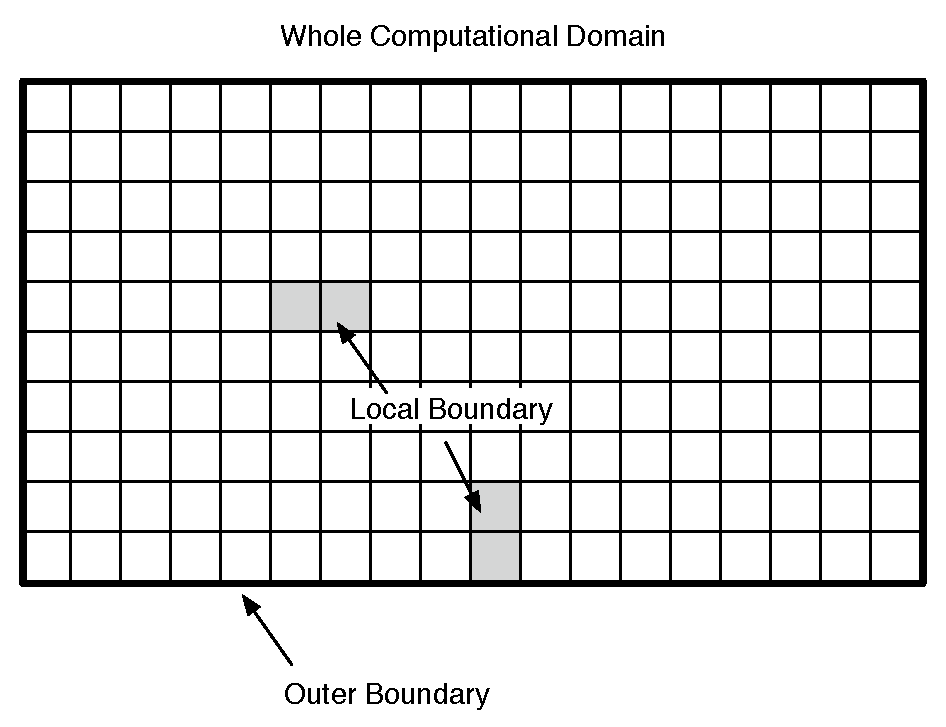
\includegraphics[width=10cm,clip]{Boundary.eps}
\end{center}
\caption{計算領域における外部境界と局所境界の指定場所}
\label{fig:BCs}
\end{figure}


%
\subsection{BC\_Tableセクションのパラメータ構造}

BC\_Tableセクションでは,次のように局所境界条件LocalBoundary\index{LocalBoundary}と外部境界条件OuterBoundary\index{OuterBoundary}の2つを記述します.

{\small
\begin{program}
BC_Table {

  LocalBoundary {
    BC[@] {
      class           = "Specified_Velocity"
      alias           = "Blower"
      type            = "velocity"
      profile         = "constant"
      velocity        = 3.4
      Normal          = (-1.0, 0.0, 0.0)
      Fluid_direction = "same_side_of_normal"
      frequency       = 0.0
      initial_phase   = 0.0
      constant_bias   = 0.0
      temperature     = 35.0
    }
  } //LocalBoundary

  OuterBoundary {
      
    // 境界条件候補リスト
    Basic_BCs[@] {
      alias    = "outer_wall"
      class    = "Wall"
      Type     = "fixed"
    }
    Basic_BCs[@] {
      alias    = "slide_wall"
      class    = "wall"
      Type     = "slide"
      Profile  = "Constant"
      Normal   = (1.0, 0.0, 0.0)
      Velocity = 1.0
    }
    Basic_BCs[@] {
      alias    = "inlet_2"
      class    = "Specified_Velocity"
      Profile  = "Constant"
      Normal   = (1.0, 0.0, 0.0)
      velocity = 5.0
    }
    Basic_BCs[@] {
      alias    = "outflow_1"
      class    = "Outflow"
      velocity_Type = "Average"
    }
      
    //外部境界条件
    Face_BC {
      X_minus {
        kind   = "inlet_2"
        medium_on_guide_cell = "air"
      }
      X_plus {
        kind   = "outflow_1"
        medium_on_guide_cell = "air"
      }
      Y_minus {
        kind   = "outer_wall"
        medium_on_guide_cell = "Fe"
      }
      Y_plus {
        kind   = "outer_wall"
        medium_on_guide_cell = "Fe"
      }
      Z_minus {
        kind   = "outer_wall"
        medium_on_guide_cell = "Fe"
      }
      Z_plus {
        kind   = "slide_wall"
        medium_on_guide_cell = "Fe"
      }
    }

  } // OuterBoundary

} // BC_Table
\end{program}
}


%
\subsection{OuterBoundary}

\hypertarget{tgt:outer_boundary}{計算領域の外部境界条件}を次の方針により指定します.

\begin{enumerate}
\item 候補となる境界条件の種類をBasic\_BCsタグ内にリストアップし,基本リストを作成します.境界条件の基本リスト\index{きほんりすと@基本リスト!きょうかいじょうけんの@境界条件の---}には,classに\textbf{表\ref{tbl:outer BC physical}}に示すキーワードを与え,aliasにユニークなラベルを与えます.
\item Face\_BCタグ内において,境界条件の基本リストのaliasラベルを参照してkindラベルに指定し,計算領域の外部境界の各面における境界条件を指定します.同時に,各面のガイドセルのセルIDをmedium\_on\_guide\_cellにより指定します.
\end{enumerate}

前述の例では,境界条件の候補として\verb|class=Wall, Specified_Velocity, Outflow|の3種類がリストアップされています.
Xマイナス方向の外部境界面に流入条件(inlet\_2)を与え,Xプラス方向の外部境界面に流出境界条件(outflow\_1),それ以外の面には壁面条件(outer\_wall, slide\_wall)を与えています.
各外部境界面のガイドセルにはmedium\_on\_guide\_cellによって,媒質をラベルで付与しています.
このラベルは,\hyperlink{tgt:medium_table}{Medium\_Table}セクションにリストアップされた媒質ラベルを参照します.
外部境界条件は,計算領域を構成する外部境界面の各面ごとに一様な境界条件となります.

指定できる境界条件の種類を\textbf{表\ref{tbl:outer BC physical}}に示します.
熱流れの場合には,壁面境界の場合に細かい指定が可能です.

\begin{table}[htdp]
\caption{外部境界で指定できる流れと熱の境界条件の種類}
\begin{center}
\small
\begin{tabular}{ll|ll} \toprule
流れの境界指定のラベル名 &  流れの境界条件 & 熱境界指定のラベル名 & 熱境界条件\\ \midrule
Outflow & 流出境界 & $\leftarrow$ & 対流流出\\
Periodic & 周期境界 & $\leftarrow$ & 周期境界\\
Specified\_Velocity & 流入境界 & Temperature & 流入温度指定\\
Symmetric & 対称境界 & $\leftarrow$ & 対称境界\\
Traction\_Free & 遠方境界 & Ambient\_Temperature & 遠方温度指定\\
Far\_Field & 遠方境界 & Ambient\_Temperature & 遠方温度指定 *テスト実装\\ \hline
Wall & 壁面境界 & Adiabatic & 断熱指定\\
& & HeatFlux & 熱流束指定\\ 
& & HeatTransfer Type\_S & 熱伝達係数と表面温度から熱伝達を計算\\
& & HeatTransfer Type\_SF & 強制対流の層流・乱流熱伝達境界\\
& & HeatTransfer Type\_SN & 自然対流の乱流熱伝達境界\\
& & HeatTransfer Type\_B & 固体壁からの放熱条件\\
& & IsoThermal & 等温指定\\
\bottomrule
\end{tabular}
\end{center}
\label{tbl:outer BC physical}
\end{table}


%
\pagebreak
\subsection{LocalBoundary}

\hypertarget{tgt:localboundary}{計算領域内に存在する局所的な境界条件}を記述するセクションで,\textbf{表\ref{tbl:tag_ibc}}に示す種類を指定できます.
FFV-Cソルバーは,局所境界条件をコンポーネント\index{コンポーネント}として扱います.
局所境界条件を指定する位置には,セル要素に対して作用するものとセル界面に作用する2種類のコンポーネントがあります.

局所境界条件の位置と形状は,解析幾何形状モデルに与えられたラベルにより判断します.
また,境界条件の詳細は,LocalBoundaryセクションの対応するラベルに記述します.
局所境界条件で指定する各コンポーネントの個数と実際の解析モデル中のコンポーネントの個数は一致している必要があります.
\textbf{指定できる局所境界条件の数は30個が上限}です.
また,\textbf{指定境界条件数と媒質数の和は30個以下}となります\footnote{これらの制限は,境界条件を効率よく実装する方法の制約から来るものです.}.

Inactiveタグは,計算空間内で計算しない不活性セルを指定します.
Cell\_Monitorは境界条件ではありませんが,境界条件と同じ指定方法を用いて実装しているので,このセクションに設けています.


\begin{table}[htdp]
\caption{局所境界条件(コンポーネント)の種類}
\begin{center}
\small
\begin{tabular}{lllll} \toprule
ラベル名 & 指定位置 & 計算モード & 実装形式 & コンポーネントの説明\\ \midrule
Specified\_Velocity & セル界面 & 流れ・熱流れ & 対流流束 & 速度指定境界\\
Outflow & セル界面 & 流れ・熱流れ & 対流流束 & 流出境界\\
Periodic & セル界面 & 流れ・熱流れ & 参照値指定 & 部分周期境界\\
%FORCING & Direct ForcingによるImmersed Boundary境界条件\\
%HEX & 熱交換器\\
%FAN & ファン\\
%DARCY & ダルシー則\\
Inactive & セル要素 & 流れ・熱流れ & マスク & 不活性化する計算空間内のセルIDを指定\\
Cell\_Monitor & セル要素 & 流れ・熱流れ & - & 物理量のモニター位置の指定\\ 
Adiabatic & セル界面 & 熱流れ & 熱流束マスク & 断熱セル指定\\
Direct\_Heat\_Flux & セル界面 & 熱流れ & 熱流束 & 熱流束指定\\
HeatTransfer\_B & セル界面 & 固体伝熱 & 熱流束 & 固体壁からの放熱条件\\
HeatTransfer\_S & セル界面 & 熱流れ & 熱流束 & 熱伝達係数と表面温度により計算\\
%HeatTransfer\_N & セル界面 & 熱 & 熱流束 & 熱伝達形式\\
HeatTransfer\_SF & セル界面 & 熱流れ & 熱流束 & 強制対流の層流・乱流熱伝達境界\\
HeatTransfer\_SN & セル界面 & 熱流れ & 熱流束 & 自然対流の乱流熱伝達境界\\
IsoThermal & セル界面 & 熱流れ & 熱流束 & 等温面指定\\
Heat\_Source & セル要素 & 熱流れ & 外力項 & 吸発熱指定\\
Specified\_Temperature & セル要素 & 熱流れ & 温度指定 & セルの温度指定\\
\bottomrule
\end{tabular}
\end{center}
\label{tbl:tag_ibc}
\end{table}


%
\pagebreak
\subsection{計算格子と内部・外部領域}

非圧縮性流体の境界条件で参照する\hypertarget{tgt:grid_arrangement}{計算領域と格子配置}について説明します.
計算領域とコロケート変数配置\index{へんすうはいち@変数配置!コロケート@Collocated---}の変数のインデクス\index{インデクス}の表記を\textbf{図\ref{fig:index_domain}},\textbf{図\ref{fig:index_cc}}に示します.

\begin{figure}[htdp]
  \begin{center}
  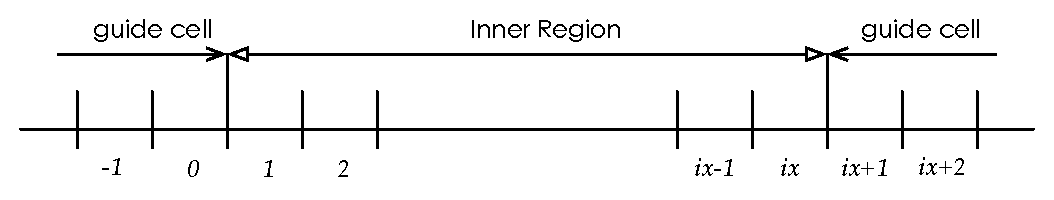
\includegraphics[width=12cm,clip]{index_domain.eps}
  \end{center}
  \caption{計算領域のインデクス}
  \label{fig:index_domain}
\end{figure}

\begin{figure}[htdp]
  \begin{center}
  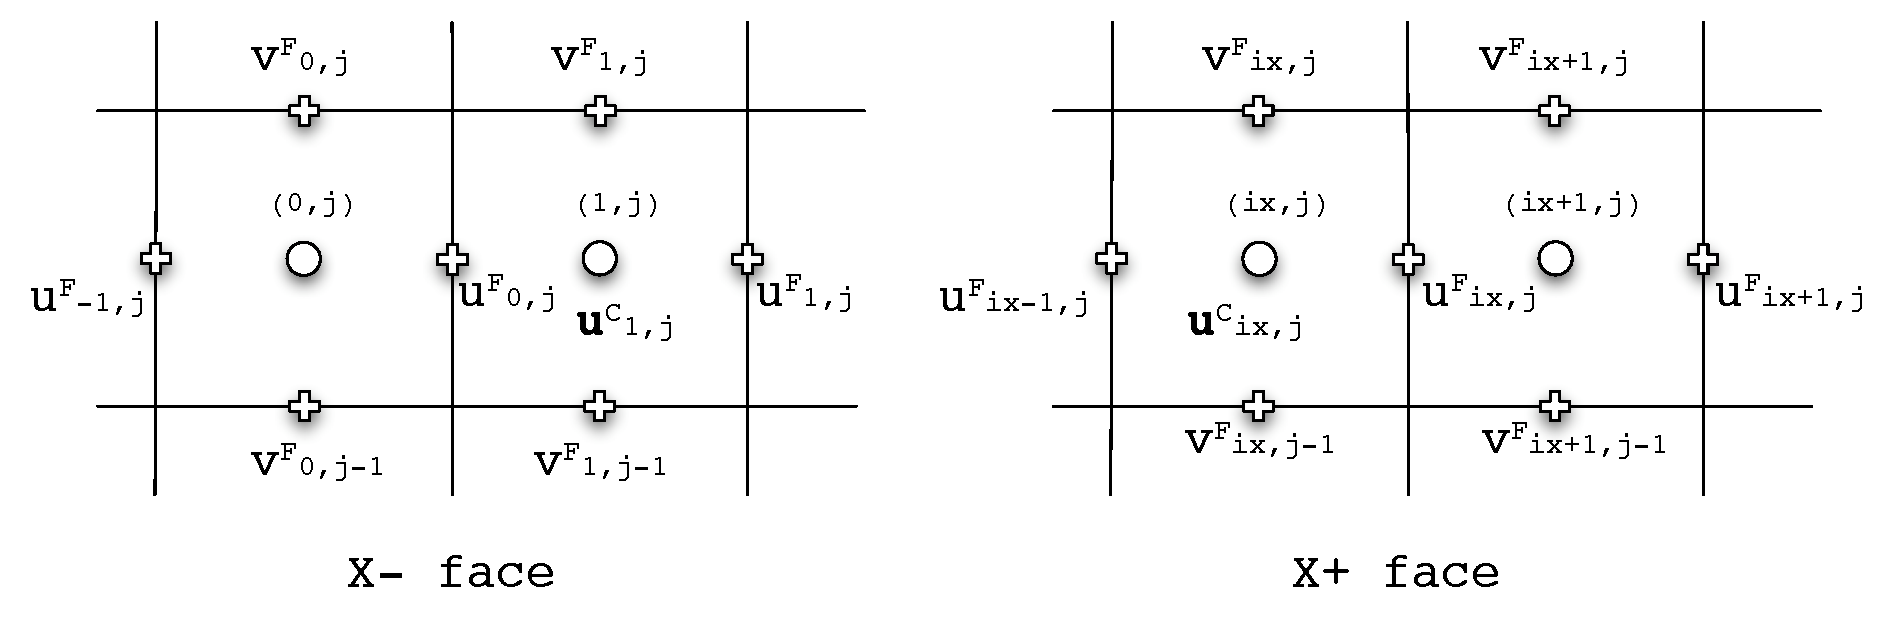
\includegraphics[width=14cm,clip]{index_cc.eps}
  \end{center}
  \caption{コロケート配置の変数のインデクス.基本変数($u_{\,i}^{\,C},\, p,\,\theta$)は全てセルセンタ位置に配置され,補助的な速度ベクトル$u_{\,i}^{\,F}$がスタガード位置に配置されます.}
  \label{fig:index_cc}
\end{figure}



%%%
\pagebreak
\section{外部境界条件}

%
\subsection{壁面境界}

\subsubsection{流れの境界条件}

壁面の速度境界条件では,指定する境界面の移動速度を与えます.
壁面速度が時間的に変化する場合と一定の場合があります.
ただし,壁面速度ベクトルは壁面と平行なスライド成分のみで,壁面と垂直な成分はゼロである点に注意します.

壁面境界は,与えられた速度からセルフェイス位置の運動量流束を計算して,運動量流束を直接与えます.
外部境界では下記のような入力パラメータで指定します.
次の境界条件の例では,Y方向に7[m/s],2[Hz]で平行振動する壁の境界条件を指定しています.

{\small
\begin{program}
OuterBoundary {
  Basic_BCs[@] {
    alias         = "sine_wall"
    class         = "Wall"
    Type          = "slide"
    Normal        = (0.0, 1.0, 0.0)
    Profile       = "Harmonic"
    amplitude     = 7.0
    frequency     = 2.0
    initial_phase = 0.0
    constant_bias = 0.0
  }
}
\end{program}
}

\begin{table}[htdp]
\caption{壁面の速度境界条件の指定パラメータ}
\begin{center}
\small
\begin{tabular}{lll} \toprule
ラベル & 指定ラベル名 & パラメータの説明\\ \midrule
Normal & | & 法線ベクトルの成分\\
Profile & Constant $|$ Harmonic & 指定速度のタイプ\\
Velocity & | & 指定単位 $[m/s]$,Profile=constantの場合のみ\\
Amplitude & | & 速度,以下のパラメータはProfile=harmonicの場合のみ\\
Frequency & | & 周波数 $f\, [Hz]$\\
Initial\_Phase & | & 初期位相 $\phi\, [Rad]$\\
Constant\_Bias & | & 一定値 $b\, [m/s]$\\
\bottomrule
\end{tabular}
\end{center}
\label{tbl:wall parameter out}
\end{table}

壁面の速度境界の指定パラメータを\textbf{表\ref{tbl:wall parameter out}}に示します.
時間変化を伴う速度指定はProfile=\lq\lq Harmonic\rq\rq を指定し,\textbf{式(\ref{eq:harmonic out})}の形式の単振動\index{たんしんどう@単振動}の境界条件を周期や初期位相,固定バイアスと供に与えます.時間的に変化しない壁面境界の場合にはProfile=\lq\lq Constant\rq\rq を指定し,周波数,初期位相,固定バイアス値の指定は不要です.

\begin{equation}
V \,{=}\, A \sin \left( 2 \mathrm{\pi} ft \,+\, \phi \right) \,+\, b
\label{eq:harmonic out}
\end{equation}


壁面境界に対する圧力の境界条件は,Navier-Stokes方程式からNeumann型の圧力境界条件が得られます.
高レイノルズ数流れにおいては,粘性項の寄与が小さいと仮定し粘性項を省略し$\nabla p=0$の形式になります.
圧力の壁面境界条件については,内部と外部の扱いは同じで,スキーム中で壁面を認識し$\nabla p=0$が満たされるようになっていますので,明示的な境界条件の指定は必要ありません.

%
\subsubsection{熱境界条件}
計算領域の外部面における壁面に対する熱境界条件としては,断熱,熱流束,熱伝達,等温が指定できます.
熱伝達境界は,さらに幾つかの指定パターンがあります.
詳細はInside\_FFVC.pdfをご覧ください.

%
\paragraph{断熱境界}
熱流束がゼロ,つまり$q^{\prime}=0$を指定します.
下記の例では,固定壁(壁面速度がゼロ)で,断熱条件を指定しています.

{\small
\begin{program}
OuterBoundary {
  Basic_BCs[@] {
    alias            = "Eng_Block"
    class            = "Wall"
    Type             = "Fixed"
    heat_type        = "Adiabatic"
    neighbor_medium  = "air-100c"
  }
}
\end{program}
}

%
\paragraph{熱流束境界}
境界面で指定の熱流束$q^{\prime}[W/m^2]$を与えます.
符号は計算領域内に流入する熱流束の場合に正,流出する熱流束の場合に負とします.
下記の例ではid=1の条件として,$12.0[W/m^2]$で流入する熱流束をもつ面を指定しています.

{\small
\begin{program}
OuterBoundary {
  Basic_BCs[@] {
    alias            = "Eng_Block"
    class            = "Wall"
    Type             = "Fixed"
    heat_type        = "heatflux"
    heat_flux        = 12.0
  }
}
\end{program}
}


%
\hypertarget{tgt:heat-transfer}{\paragraph{熱伝達境界}}
熱伝達境界は次式の形式で熱流束を与える条件で,幾つかの種類があります.
熱流体解析のモードと指定できる熱伝達境界の関係を\textbf{表\ref{tbl:type of HT}}に示します.

\begin{table}[htdp]
\caption{熱伝達境界条件とKind\_of\_Solverの関係}
\begin{center}
\small
\begin{tabular}{ll} \toprule
KIND\_OF\_SOLVER & 指定できる熱伝達境界の種類\\ \midrule
FLOW\_ONLY & -\\
THERMAL\_FLOW $|$ THERMAL\_FLOW\_NATURAL & Type\_S $|$ Type\_SN $|$ Type\_SF\\
CONJUGATE\_HEAT\_TRANSFER & Type\_N\\
SOLID\_CONDUCTION & Type\_B\\ \bottomrule
\end{tabular}
\end{center}
\label{tbl:type of HT}
\end{table}


\begin{equation}
q^{\prime} \,=\, -H(\theta_{sf}^{\prime}\,-\,\theta_{\infty}^{\prime})
\label{eq:ht form}
\end{equation}

\begin{center}
\begin{tabular}{lll}
$H$ &  $[W\,/\,(m^2K)]$ & Coefficient\, of\, heat\, transfer\\
$\theta_{sf}^{\prime}$ & $[K]$ & Surface\, temperature\, of\, solid\\
$\theta_{\infty}^{\prime}$ & $[K]$ & Temperature\, at\, outer\, boundary\, layer\\
\end{tabular}
\end{center}

\vspace{5mm}
\begin{indentation}{3zw}{0zw}

%
\subparagraph{Type\_S  表面温度と熱伝達係数により計算}
Type\_Sは表面温度と熱伝達係数を与え,熱流束を計算します.
\textbf{式(\ref{eq:ht form})}において,熱伝達係数$H$と固体表面温度$\theta_{sf}^{\prime}$を与え,\textbf{図\ref{fig:HT_Type_S}}に示す固体表面に隣接する流体セルの値を$\theta_{\infty}^{\prime}$として,界面での熱流束を計算します.

\begin{figure}[htdp]
\begin{center}
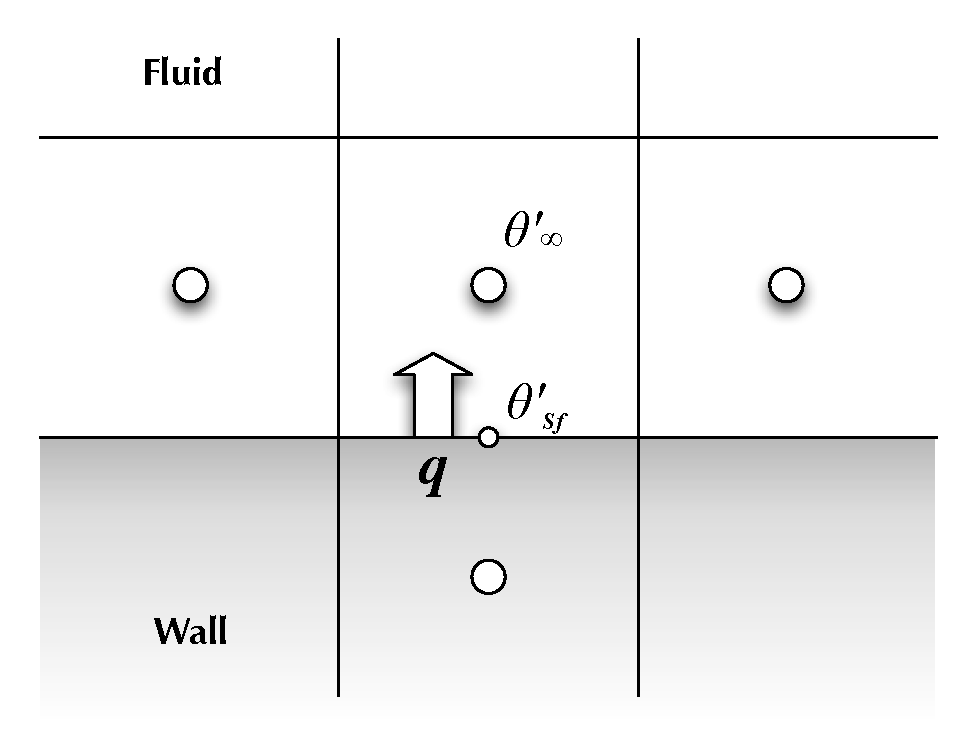
\includegraphics[width=7cm,clip]{HeatTransfer_Type_S.eps}
\end{center}
\caption{Type\_Sの熱伝達境界}
\label{fig:HT_Type_S}
\end{figure}

以下に,熱境界部分のみパラメータ指定の一例を示します.

{\small
\begin{program}
OuterBoundary {
  Basic_BCs[@] {
    alias                 = "Exhaust"
    class                 = "Wall"
    Type                  = "Fixed"
    heat_type             = "HeatTransfer_S"
    Surface_Temperature   = 300.0
    Coef_of_Heat_Transfer = 20.0
  }
}
\end{program}
}

\begin{table}[htdp]
\caption{熱伝達境界Type\_Sの指定パラメータ}
\begin{center}
\small
\begin{tabular}{ll} \toprule
指定キーワード & パラメータの説明\\ \midrule
Coef\_of\_Heat\_Transfer & 熱伝達係数$[W/(m^2K)]$\\
Surface\_Temperature & 表面温度$[K\,|\,{}^\circ\mathrm{C}]$\\
\bottomrule
\end{tabular}
\end{center}
\label{tbl:hts}
\end{table}

%
\subparagraph{Type\_SN  自然対流の乱流熱伝達}
自然対流の場合の乱流熱伝達の実験式を実装した境界条件です.
文献\cite{shouji:95:Dennetsu}には,平板に対する自然対流の層流と乱流の熱伝達に関する近似式が説明されています.
雰囲気流体の温度に比べ加熱面の温度が非常に高い場合,平板が長くなると境界層が不安定になり,ほぼ$Ra>10^9$で層流から乱流へ遷移します.
垂直平板に関する平均熱伝達$(\overline{Nu_L},代表長L)$は次式で整理されます.

\begin{equation}
\left.
\begin{array}{lll}
\vspace{1mm}
層流 & \overline{Nu_L} \,=\, 0.59Ra_L^{1/4} & (10^4 < Ra_L < 10^9)\\
乱流 & \overline{Nu_L} \,=\, 0.10Ra_L^{1/3} & (10^9 < Ra_L < 10^{13})
\end{array} \right\}
\label{eq:natural_convection_vert_ht}
\end{equation}

一方,水平平板の場合には,加熱面が上面と下面にある場合で雰囲気流体の挙動が異なるため,\textbf{式(\ref{eq:natural_convection_horiz_ht})}のように整理されています.

\begin{equation}
\left.
\begin{array}{lll}
\vspace{1mm}
上面加熱 & \overline{Nu_L} \,=\, 0.54Ra_L^{1/4} & (10^4 < Ra_L < 10^7)\\
\vspace{1mm}
上面加熱 & \overline{Nu_L} \,=\, 0.15Ra_L^{1/3} & (10^7 < Ra_L < 10^{11})\\
\vspace{1mm}
下面加熱 & \overline{Nu_L} \,=\, 0.27Ra_L^{1/4} & (10^5 < Ra_L < 10^{10})
\end{array} \right\}
\label{eq:natural_convection_horiz_ht}
\end{equation}

上式を形式的にまとめると,

\begin{equation}
H \,=\, \alpha Ra_L^\beta \frac{\lambda}{L^\prime}
\label{eq:typeSN_form_ht}
\end{equation}

Type\_SNの境界条件は,上式のパラメータを実装しています.ここでは,垂直平板と水平平板の上面は,同じ係数を用いています.

{\small
\begin{program}
OuterBoundary {
  Basic_BCs[@] {
    alias                    = "Exhaust"
    class                    = "Wall"
    Type                     = "Fixed"
    heat_type                = "HeatTransfer_SN"
    Surface_Temperature      = 100.0
    Ref_Temp_Mode            = "Bulk_Temperature"
    vertical_laminar_alpha   = 0.59
    vertical_laminar_beta    = 0.25
    vertical_turbulent_alpha = 0.1
    vertical_turbulent_beta  = 0.3333333
    vertical_Ra_critial      = 1.0e9
    lower_laminar_alpha      = 0.27
    lower_laminar_beta       = 0.25
    lower_turbulent_alpha    = 0.27
    lower_turbulent_beta     = 0.25
    lower_Ra_critial         = 1.0e9
  }
}
\end{program}
}

\begin{table}[htdp]
\caption{熱伝達境界Type\_SNのパラメータ}
\begin{center}
\small
\begin{tabular}{ll}\toprule
パラメータタグ & 記号の意味\\ \midrule
Vertival\_Laminar\_Alpha & 垂直平板と水平平板(上面)の層流時の係数$\alpha$\\
Vertival\_Laminar\_Beta & 垂直平板と水平平板(上面)の層流時の係数$\beta$\\
Vertival\_Turbulent\_Alpha & 垂直平板と水平平板(上面)の乱流時の係数$\alpha$\\
Vertival\_Turbulent\_Beta & 垂直平板と水平平板(上面)の乱流時の係数$\beta$\\
Vertival\_Ra\_Critial & 垂直平板と水平平板(上面)の臨界Ra数$Ra_L$\\
Lower\_Laminar\_Alpha & 水平平板(下面)の層流時の係数$\alpha$\\
Lower\_Laminar\_Beta & 水平平板(下面)の層流時の係数$\beta$\\
Lower\_Turbulent\_Alpha & 水平平板(下面)の乱流時の係数$\alpha$\\
Lower\_Turbulent\_Beta & 水平平板(下面)の乱流時の係数$\beta$\\
Lower\_Ra\_Critial & 水平平板(下面)の臨界Ra数$Ra_L$\\ 
Ref\_Temp\_Mode & Bulk\_Temperature or Local\_Temperature\\ \bottomrule
\end{tabular}
\end{center}
\label{tbl:htsn}
\end{table}


%
\subparagraph{Type\_SF  強制対流の層流・乱流熱伝達}
強制対流の場合の層流・乱流熱伝達の実験式を実装した境界条件です.
文献\cite{shouji:95:Dennetsu}から,平板に対する発達した強制対流の乱流熱伝達は,実験による摩擦係数の測定結果とチルトン-コルバーンのアナロジーを用い,温度一定で平板が遷移長さよりも十分に大きいと仮定すると,\textbf{式(\ref{eq:forced_convection_ht})}のように表せます.
実験式を整理すると,熱伝達係数は以下のような表現ができます.

\begin{equation}
\overline{Nu_L} \,=\, 0.037Re_L^{4/5}Pr^{1/3}
\label{eq:forced_convection_ht}
\end{equation}

形式的に次式のように表し,パラメータを求めます.

\begin{equation}
H \,=\, \alpha Re_L^\beta \, Pr^\gamma \, \frac{\lambda}{L^\prime}
\label{eq:typeSF_form_ht}
\end{equation}


温度差の定義にはバルク温度と隣接セルの値を用いたオプションが選択できます.
以下に,パラメータ指定の一例を示します.

{\small
\begin{program}
OuterBoundary {
  Basic_BCs[@] {
    alias               = "Exhaust"
    class               = "Wall"
    Type                = "Fixed"
    heat_type           = "HeatTransfer_SF"
    Surface_Temperature = 500.0
    Ref_Temp_Mode       = "Bulk_Temperature"
    alpha               = 0.037
    beta                = 0.8
    gamma               = 0.333333
  }
}
\end{program}
}

\begin{table}[htdp]
\caption{熱伝達境界Type\_SFのパラメータ}
\begin{center}
\small
\begin{tabular}{ll}\toprule
タグ & 記号の意味\\ \midrule
alpha & \textbf{式(\ref{eq:typeSF_form_ht})}中の係数$\alpha$\\
beta & 係数$\beta$\\
gamma & 係数$\gamma$\\
Ref\_Temp\_Mode & Bulk\_Temperature or Local\_Temperature\\ \bottomrule
\end{tabular}
\end{center}
\label{tbl:htsf}
\end{table}


%
\subparagraph{Type\_B  固体壁からの放熱条件}
熱伝達係数とバルク温度を与え,熱流束を計算します.固体の熱移動のみを解く場合の境界条件として利用します.
以下に,パラメータ指定の一例を示します.

{\small
\begin{program}
OuterBoundary {
  Basic_BCs[@] {
    alias                 = "Exhaust"
    class                 = "Wall"
    Type                  = "Fixed"
    heat_type             = "HeatTransfer_B"
    Coef_of_Heat_Transfer = 0.12
    Bulk_Temperature      = 500.0
  }
}
\end{program}
}

\begin{table}[htdp]
\caption{熱伝達境界Type\_Bの指定パラメータ}
\begin{center}
\small
\begin{tabular}{ll} \toprule
指定キーワード & パラメータの説明\\ \midrule
Coef\_of\_Heat\_Transfer & 熱伝達係数 $[W/(m^2K)]$\\
Bulk\_Temperature & 境界層外層温度 $[K\,|\,{}^\circ\mathrm{C}]$\\
\bottomrule
\end{tabular}
\end{center}
\label{tbl:htb}
\end{table}

\end{indentation}


%
\paragraph{等温境界}

等温壁境界は,指定面で温度が一定となる境界条件で,面温度を一定に保つような熱流束が発生します.
例えばXマイナス側の外部境界面のセル界面位置では,次の形式の熱流束となります.

\begin{equation}
q^{\prime}_{ISO,\,1/2} \,=\, -\mathit{\lambda}_1 \frac{\mathit{\theta}^{\prime}_1 - \mathit{\theta}^{\prime}_{sf}} {h^{\prime}\slash{2}}
\label{eq:qiso1}
\end{equation}

{\small
\begin{program}
OuterBoundary {
  Basic_BCs[@] {
    alias            = "Exhaust"
    class            = "Wall"
    Type             = "Fixed"
    heat_type        = "IsoThermal"
    Temperature      = 100.0
  }
}
\end{program}
}

\begin{table}[htdp]
\caption{等温壁の指定パラメータ}
\begin{center}
\small
\begin{tabular}{ll} \toprule
指定キーワード & パラメータの説明\\ \midrule
Temperature & 表面温度 $[K\,|\,{}^\circ\mathrm{C}]$\\
\bottomrule
\end{tabular}
\end{center}
\label{tbl:iso-thermal}
\end{table}


%%%
\pagebreak
\subsection{対称境界}

外部境界にのみ用いられる境界条件で,指定する面が対称面であると仮定します.\textbf{図\ref{fig:symmetric plane}}にXプラス方向の境界面における対称境界面の速度ベクトルの境界条件を示します.速度については,面直な成分のみ固体壁と同じで,残りはフリーとします.圧力は勾配がゼロとします.


{\small
\begin{program}
OuterBoundary {
  Basic_BCs[@] {
    alias    = "left_side"
    class    = "Symmetric"
  }
}
\end{program}
}


上記の例では,aliasにleft\_sideというラベル名を与え,対称境界条件を指定しています.

\begin{figure}[htbp]
\begin{center}
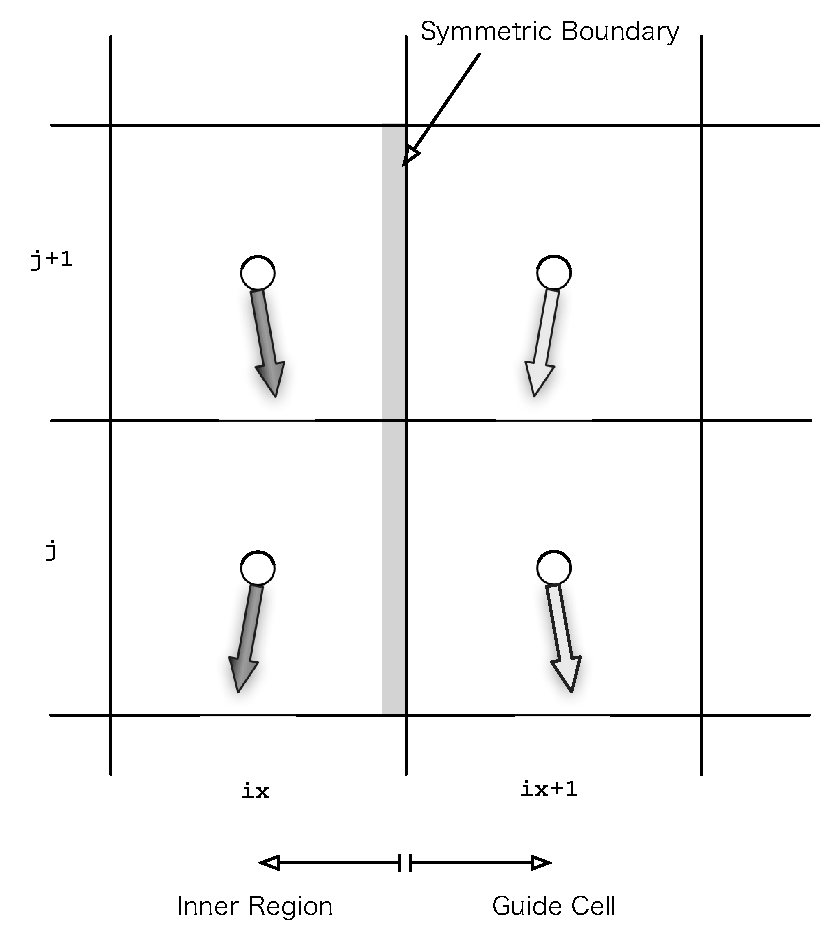
\includegraphics[width=7cm,clip]{symmetric.eps}
\end{center}
\caption{対称境界面における境界条件}
\label{fig:symmetric plane}
\end{figure}

熱計算では,対称境界が指定された面は断熱境界となります.


%%%
\pagebreak
\subsection{流出境界}

流出境界を指定する場合には,流出方向は既知とします.
外部境界では\textbf{図\ref{fig:outflow BC outer}}に示すようにガイドセルのセル属性は流体であることが必要です.
ガイドセルのセル属性の指定方法については\hyperlink{tgt:outer_boundary}{OuterBoundary}を参照してください.

{\small
\begin{program}
OuterBoundary {
  Basic_BCs[@] {
    alias    = "to_exhaust"
    class    = "outflow"
    velocity_type = "minmax"
  }
}
\end{program}
}

\begin{figure}[htbp]
\begin{center}
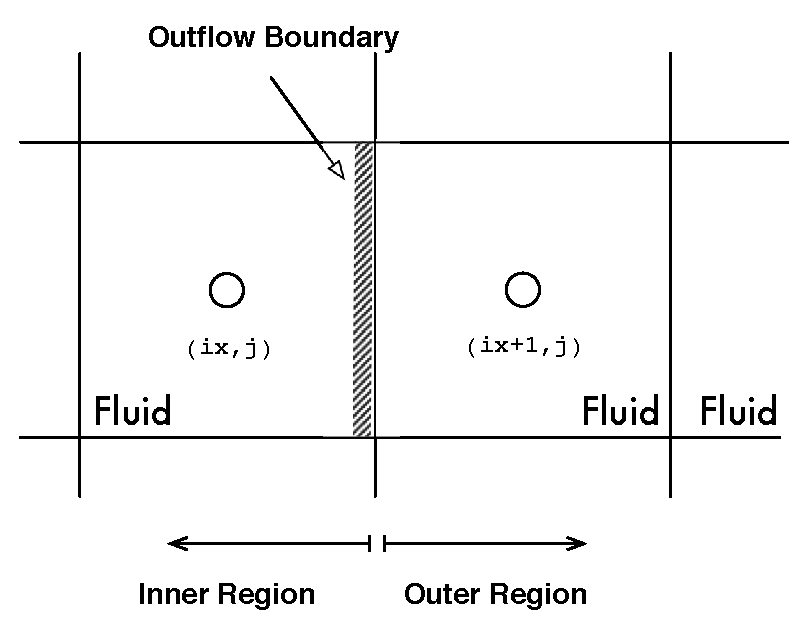
\includegraphics[width=8cm,clip]{outflowBC_outer.eps}
\end{center}
\caption{外部境界面における流出境界.x+方向の例.}
\label{fig:outflow BC outer}
\end{figure}

\noindent 指定するパラメータとして,対流流出速度の評価方法があります.この例では,流出速度の評価方法にMinmaxを指定しています.
流出速度の選び方として,流出断面の平均速度や最大値と最小値の算術平均などが提案されており,経験上,内部流の場合にはAverageが流出速度のよい近似値を与えます.
一方,外部流や噴流のような無限空間の境界面の場合にはMinMaxがよい近似値となります.
流出速度の指定は,\textbf{表\ref{tbl:outflow velocity}}のようにVelocity\_TypeタグにてAverage または Minmaxを指定します.
Averageは,物体でブロックされていない有効セルの平均値をとります.
Minmaxは,境界面における有効セルの流速の最大値と最小値の算術平均値を与えます.

\begin{table}[htdp]
\caption{対流流出速度の評価方法の指定}
\begin{center}
\small
\begin{tabular}{ll} \toprule
Velocity\_Type & パラメータの説明\\ \midrule
Average & 流出面の有効セルに対する平均値\\
Minmax & 流出面の有効セルに対する最大値と最小値の算術平均値\\ \bottomrule
\end{tabular}
\end{center}
\label{tbl:outflow velocity}
\end{table}

圧力境界条件としては,Fractional Step法のアルゴリズムに適合するように,境界面上で$\nabla p=0$を用いています.

熱境界としても,速度と同様に,対流流出型の境界条件となります.



%%
\pagebreak
\subsection{速度指定境界}

この境界条件は,セル界面における運動量流束の形で実装されています.
まず,速度指定境界のパラメータについて説明します.

{\small
\begin{program}
OuterBoundary {
  Basic_BCs[@] {
    alias    = "inlet"
    class    = "Specified_Velocity"
    Profile  = "Harmonic"
    Normal   = (0.0, 1.0, 0.0)
    amplitude= 7.0
    frequency= 2.0
    initial_phase = 0.0
    constant_bias = 0.0
    Temperature = 30.0
  }
}
\end{program}
}

\noindent 境界面の指定方法は,\textbf{表\ref{tbl:vspec parameter with heat}}に示すパラメータを与えます.
時間変化を伴う速度指定はProfile=\lq\lq Harmonic\rq\rq を指定し,\textbf{式(\ref{eq:harmonic out})}の形式の単振動の境界条件を周期や初期位相,固定バイアスと供に与えます.時間的に変化しない壁面境界の場合にはProfile=\lq\lq Constant\rq\rq を指定し,周波数,初期位相,固定バイアス値の指定は不要です.

圧力の境界条件は,壁面境界条件と同様にNeumann型の圧力境界条件$\nabla p=0$が用いられます.

温度の指定単位は,Unitセクションの\hyperlink{tgt:unit}{Temperature}で指定した単位になります.

\begin{table}[htdp]
\caption{速度指定境界のパラメータ}
\begin{center}
\small
\begin{tabular}{lll} \toprule
ラベル & 指定キーワード & パラメータの説明\\ \midrule
Normal & | & 法線ベクトルの成分\\
Velocity & | & 指定単位 $[m/s]$,Profile=constantの場合のみ\\
Amplitude & | & 速度,以下のパラメータはProfile=harmonicの場合のみ\\
Frequency & | & 周波数 $f\, [Hz]$\\
Initial\_Phase & | & 初期位相 $\phi\, [Rad]$\\
Constant\_Bias & | & 一定値 $b\, [m/s]$\\
Temperature & | & 指定温度 $[K\,|\,{}^\circ\mathrm{C}]$\\
\bottomrule
\end{tabular}
\end{center}
\label{tbl:vspec parameter with heat}
\end{table}


%%
\pagebreak
\subsection{周期境界}

\hypertarget{tgt:preriodic}{周期境界条件}には,外部境界に対する周期境界と計算内部領域に設定する部分的な周期境界条件を併用する条件の2種類があります.
外部境界に対する周期境界条件では,\textbf{図\ref{fig:index_domain}}において,Inner\,Regionの両端の境界が重なる状態を想定しています.

\vspace{2mm}

外部境界に対する周期境界条件には\textbf{表\ref{tbl:periodic mode}}に示す3つのモードが指定できます.
下記には,各モードの例を示します.
Simple\_Copyモードは,周期境界条件面の両端で,単純に計算内部領域の値を他方のガイドセルにコピーします.
Pressure\_Diffrenceモードは,両端で圧力差を与える周期境界条件で,速度や温度についてはSimple\_Copyモードと同じですが,圧力は指定の圧力差を与えます.上流側と下流側の設定が必要です.
Driverモードは,乱流計算などで発達したチャネル流を上流境界として与えるためのしくみで,局所境界条件との組み合わせで利用します.Driverモードの説明は局所境界条件をご覧ください.

{\small
\begin{program}
OuterBoundary {
  Basic_BCs[@] {
    alias    = "x-dir_periodic_1"
    class    = "periodic"
    Mode     = "Simple_Copy"
  }
  
  Basic_BCs[@] {
    alias    = "x-dir_periodic_2"
    class    = "periodic"
    Mode     = "Directional"
    flow_direction = "upstream"
    pressure_difference = 8.148e-3
  }
  
  Basic_BCs[@] {
    alias    = "x-dir_periodic_3"
    class    = "periodic"
    Mode     = "Directional"
    flow_direction = "downstream"
    pressure_difference = 8.148e-3
  }
  
  Basic_BCs[@] {
    alias    = "x-dir_periodic_3"
    class    = "periodic"
    Mode     = "driver"
    driver_direction = "x_minus"
  }
}
\end{program}
}

\begin{table}[htdp]
\caption{周期境界条件のモード}
\begin{center}
\small
\begin{tabular}{ll} \toprule
キーワード & モードの説明\\ \midrule
Simple\_Copy & 周期境界の両端で物理量をガイドセルにコピーします.\\
Directional  & 圧力差を与える周期境界条件で,上流と下流の境界面を指定します.\\
Driver       & 計算領域内で部分的な周期境界条件を設定します.\\ \bottomrule
\end{tabular}
\end{center}
\label{tbl:periodic mode}
\end{table}

Directionalモードでは,\textbf{表\ref{tbl:parameter dir. mode}}に示すパラメータが必要で,Pressure\_Differenceの値が,UpstreamとDownstreamで同じ値である必要があります.

\begin{table}[htdp]
\caption{Directionalモードに必要なパラメータ}
\begin{center}
\small
\begin{tabular}{ll} \toprule
必要なキーワード & パラメータの説明\\ \midrule
Pressure\_Difference & 両端にかける圧力差 $[Pa]$\\
Flow\_Direction & Upstream(上流面)または Downstream(下流面)\\
\bottomrule
\end{tabular}
\end{center}
\label{tbl:parameter dir. mode}
\end{table}



%%%
\pagebreak
\subsection{トラクションフリー境界}

遠方境界条件として,トラクションフリー条件を用います.

\vspace{2mm}

トラクションフリー条件は,外部境界に対してのみ指定できる境界条件で,計算対象の主領域から遠方の挙動を仮定した条件です.
つまり,圧力の遠方条件$p=0$(基準圧)を考慮し,計算外部境界において流体の内部応力の法線方向成分がゼロである仮定を用いています.
この境界条件は,噴流のエントレインメントの効果などを考慮できる利点がありますが,渦が流出するような境界には適用できません.

{\small
\begin{program}
OuterBoundary {
  Basic_BCs[@] {
    alias    = "ambient"
    class    = "Traction_Free"
    ambient_temperature = 25.0
  }
}
\end{program}
}

熱流れの場合には,遠方場における温度を指定します.



%%%
\pagebreak
\subsection{遠方境界}

外挿境界条件で,実験的な実装です.

\vspace{2mm}

指定された外部境界面において,外部境界面の値を内部から外挿して与えます.

{\small
\begin{program}
OuterBoundary {
  Basic_BCs[@] {
    alias    = "extrapolation"
    class    = "Far_Field"
    ambient_temperature = 25.0
  }
}
\end{program}
}

熱流れの場合には,流入時に対応する温度を指定します.



%%%-------------------------------------------------
\pagebreak
\section{局所境界条件}
内部領域の境界条件は,コンポーネントとして実装しています.
局所境界条件の多くは,計算空間内に局所的に存在し,複雑な計算処理を行います.
コンポーネントはそれらを効率よく取り扱うための機能です.
1つのセルを構成する6つの面にはそれぞれ別の境界条件を指定できますが,1つのセルには同種の流出境界は1種類だけしか設定できません.

%
\subsection{壁面境界}

\subsubsection{流れの境界条件}
計算領域内部の壁面境界条件は,モデルで固体壁に指定したセルが固体として認識され,セル界面の流束が指定する壁面速度から直接計算されるので,特に明示的な指定はありません.

壁面境界に対する圧力の境界条件は,Navier-Stokes方程式からNeumann型の圧力境界条件が得られます.
高レイノルズ数流れにおいては,粘性項の寄与が小さいと仮定し粘性項を省略し$\nabla p=0$の形式になります.
Binary近似の場合には,固体壁面との界面で$\nabla p=0$を満たすようにスキームが構成されています.

%
\subsubsection{熱境界条件}
壁面に対する熱境界条件としては,断熱,熱流束,熱伝達,等温,温度条件を指定できます.
熱境界条件の実装の詳細はInside\_FFVC.pdfをご覧ください.

%
\paragraph{熱境界条件の指定方法}
\hypertarget{tgt:spec of heat bc}{熱境界条件}は,セルの界面に与えます.多くの場合は流体と固体の界面ですが,固体熱伝導と共役熱移動の場合には,固体-固体界面の場合もあります.
局所境界の場合の界面の指定方法としては,指定する2つのIDで挟まれるボクセルの構成面を指定界面とします.
指定するIDの一つはキーIDで,主に固体セルを指定します.もうひとつのIDはDef\_Face IDです.

熱境界条件をコンポーネントとして与える場合,固体面をキーIDに指定します.
このときの熱流束の方向は,
\textbf{図\ref{fig:heat bc on solid}}において,固体面から流体側へ向かう法線をと同じ方向です.
つまり,この法線方向が指定する値の正の方向とし,流体側への熱移動を正の方向と考えます.

\begin{figure}[htbp]
\begin{center}
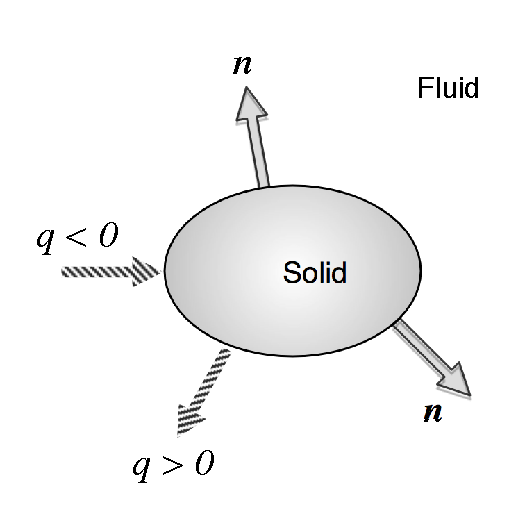
\includegraphics[width=6cm,clip]{heatBC.eps}
\end{center}
\caption{流体-固体界面における熱境界条件の熱流束の方向}
\label{fig:heat bc on solid}
\end{figure}

FFV-Cの熱流体解析には幾つかのモードがあります.\hyperlink{tgt:solver_property}{Kind\_of\_Solver}の指定モードによって,計算空間内の計算対象とする部分が異なります.
Thermal\_FlowとThermal\_Flow\_Naturalの場合は,熱流動計算で流体の温度のみを解きます\footnote{計算の実装上,固体部分も解いていますが,その値はマスクされ,無効化されています.}.したがって,固体部分は計算対象とはならず不活性セルとして扱います.これより,流体-固体の境界面で与える熱境界条件(熱流束)は,流体セル側のみに指定されます.

一方,Solid\_Conductionの場合は,固体部分の熱伝導のみを解くので,流体部分を不活性セルとして扱います.したがって,流体-固体の境界面で与える熱境界条件は,固体セル側のみに指定されます.

Conjugate\_Heat\_Transferの場合には,流体と固体の両方の熱移動を計算します.したがって,流体-固体の境界面で与える熱境界条件は,流体セルと固体セルの両方で指定されます.

以下の各境界条件の指定で述べるように,IDとDef\_Faceタグの組み合わせにより,流体-固体の境界面を指定します.
このとき,\textbf{IDには固体のIDを,Def\_Faceには流体または固体のIDを指定すること}を基本としてください\footnote{IDに固体を指定する理由は,参照範囲を小さく抑えて効率的な計算をするためです.}.

%
\paragraph{断熱境界}
断熱壁では指定面で熱流束がゼロ,つまり$q^{\prime}=0$を指定します.固体セルと流体セルの界面に何も熱境界条件を指定しなければ,断熱境界条件となります.また,明示的に次のように\lq\lq Adiabatic\rq\rq セクションで断熱面を指定することができます.

{\small
\begin{program}
LocalBoundary {
    BC[@] {
      class                    = "Adiabatic"
      alias                    = "Eng_Block"
      neighbor_medium          = "air-100c"
    }
}
\end{program}
}
この例では,ID=\lq\lq 6\rq\rq の固体セルのうち,ID=\lq\lq 3\rq\rq の流体セルに接する面に対して,断熱境界条件を指定しています.

%
\paragraph{熱流束境界}
熱流束境界は境界面で指定の熱流束を与えます.

{\small
\begin{program}
<LocalBoundary>
  <Elem name="Direct_Heat_Flux" ID="6" comment="outer_wall">
    <Param name="Def_Face"    dtype="INT"    value="3"/>
    <Param name="Heat_Flux"   dtype="REAL"   value="10.0"/>
  </Elem>
</LocalBoundary>
\end{program}
}

%
\paragraph{熱伝達境界}
熱伝達境界は次式の形式で熱流束を与える条件で,幾つかの種類があります.固体-流体セル間の熱伝達境界の与え方は,\hyperlink{tgt:heat-transfer}{外部境界条件の熱伝達境界}で説明した内容と同じです.

\begin{indentation}{3zw}{0zw}
%
\subparagraph{Type\_S  表面温度と熱伝達係数により計算}
Type\_Sは固体表面温度と熱伝達係数を与え,熱流束を計算します.
\textbf{式(\ref{eq:ht form})}において,$\theta_{\infty}^{\prime}$を固体表面に接する流体セルの値と仮定します.
以下に,熱境界部分のみパラメータ指定の一例を示します.

{\small
\begin{program}
<LocalBoundary>
  <Elem name="HeatTransfer_S" ID="6" comment="engine">
    <Param name="Def_Face"              dtype="INT"  value="3"/>
    <Param name="Surface_Temperature"   dtype="REAL" value="300.0"/>
    <Param name="Coef_of_Heat_Transfer" dtype="REAL" value="20.0"/>
  </Elem>
</LocalBoundary>
\end{program}
}

%
\subparagraph{Type\_SN  自然対流の乱流熱伝達}
自然対流の場合の乱流熱伝達の実験式を実装した境界条件です.

{\small
\begin{program}
LocalBoundary {
    BC[@] {
      class                    = "HeatTransfer_SN"
      alias                    = "Exhaust"
      neighbor_medium          = "air-100c"
      Surface_Temperature      = 500.0
      Ref_Temp_Mode            = "Bulk_Temperature"
      vertical_laminar_alpha   = 0.59
      vertical_laminar_beta    = 0.25
      vertical_turbulent_alpha = 0.1
      vertical_turbulent_beta  = 0.3333333
      vertical_Ra_critial      = 1.0e9
      lower_laminar_alpha      = 0.27
      lower_laminar_beta       = 0.25
      lower_turbulent_alpha    = 0.27
      lower_turbulent_beta     = 0.25
      lower_Ra_critial         = 1.0e9
    }
}
\end{program}
}

%
\subparagraph{Type\_SF  強制対流の層流・乱流熱伝達}
強制対流の場合の層流・乱流熱伝達の実験式を実装した境界条件です.

{\small
\begin{program}
<LocalBoundary>
  <Elem name="HeatTransfer_SF" ID="6" comment="engine">
    <Param name="Def_Face"            dtype="INT"    value="3"/>
    <Param name="Surface_Temperature" dtype="REAL"   value="500.0"/>
    <Param name="Ref_Temp_Mode"       dtype="STRING" value="Bulk_Temperature"/>
    <Param name="alpha"               dtype="REAL"   value="0.037"/>
    <Param name="beta"                dtype="REAL"   value="0.8"/>
    <Param name="gamma"               dtype="REAL"   value="0.333333"/>
  </Elem>
</LocalBoundary>
\end{program}
}

%
\subparagraph{Type\_B  固体壁からの放熱条件}
熱伝達係数とバルク温度を与え,熱流束を計算します.固体熱伝導を解く場合の境界条件として利用します.

{\small
\begin{program}
<LocalBoundary>
  <Elem name="HeatTransfer_B" ID="6" comment="engine">
    <Param name="Def_Face"              dtype="INT"    value="3"/>
    <Param name="Bulk_Temperature"      dtype="REAL"   value="500.0"/>
    <Param name="Coef_of_Heat_Transfer" dtype="REAL"   value="0.12"/>
  </Elem>
</LocalBoundary>
\end{program}
}

\end{indentation}


%
\paragraph{等温壁境界}
等温壁境界は,指定面で温度が一定となる境界条件で,面温度を一定に保つような熱流束が発生します.

{\small
\begin{program}
<LocalBoundary>
  <Elem name="IsoThermal" ID="6" comment="outer_wall">
    <Param name="Def_Face"    dtype="INT"    value="3"/>
    <Param name="Temperature" dtype="REAL"   value="100.0"/>
  </Elem>
</LocalBoundary>
\end{program}
}


%%
\subsection{流出境界条件}

\paragraph{流れの境界条件}
計算領域内部に設定する流出境界について説明します.
\textbf{局所境界の場合には流出側のセルは固体セルであり,かつ流出方向に2セル必要になること}に注意してください.
つまり,\textbf{図\ref{fig:outflow BC inner}}においては,セル$(i,\,j)$は流体,セル$(i+1,\,j)$は固体を指定します.
ハッチング部分,つまり$(i,\,j)$セルの固体セルに隣接する面が流出境界として指定されています.
計算内部領域における境界面は,次のように対象となる面をid=20とid=210の2つのIDで挟むことにより指定します.
速度の流出面における対流速度の評価方法として流出コンポーネントの平均速度を用い,流出面における圧力境界は圧力勾配ゼロとしています.

{\small
\begin{program}
<LocalBoundary> 
  <Elem name="outflow" id="20" comment="out">
    <Param name="def_face"    dtype="INT"    value="210" />
  </Elem>
</LocalBoundary>
\end{program}
}

\begin{figure}[htbp]
\begin{center}
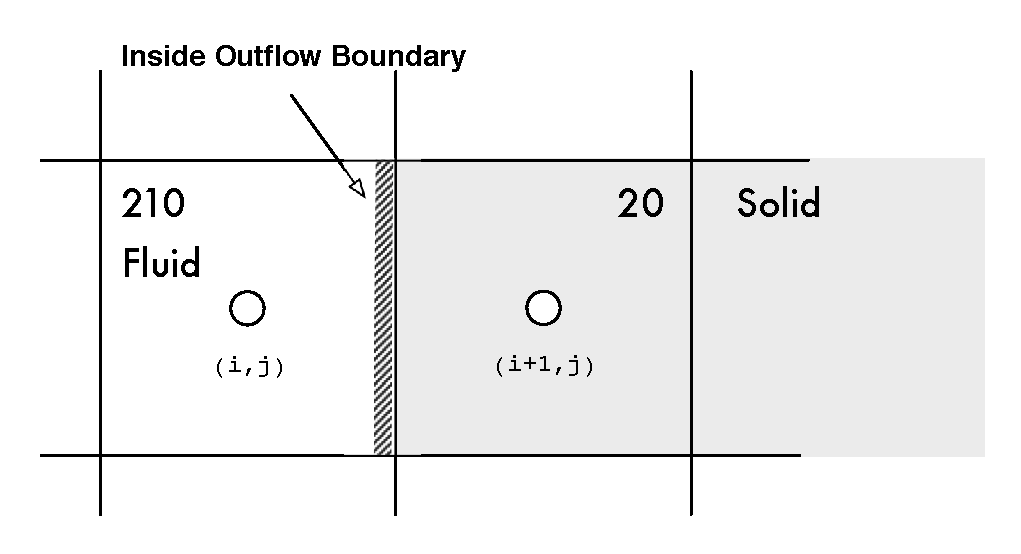
\includegraphics[width=8cm,clip]{outflowBC_inner.eps}
\end{center}
\caption{計算内部領域における流出境界の設定}
\label{fig:outflow BC inner}
\end{figure}

%
\paragraph{熱流出境界}
熱の流出境界は,流出界面の対流熱流束$\tilde{f}$を一次風上の形式で評価します.

\begin{equation}
\tilde{f} \,=\, \frac{\partial}{\partial x^{\prime}}\, \left( u^{\prime}\,\theta^{\prime} \right)_{upstream\_face}
\label{eq:outflow heat flux}
\end{equation}

分離解法において温度輸送方程式を解く過程では,速度は既知なので上式は直ちに計算できます.


%%%
\subsection{速度指定条件}

\paragraph{流れの境界条件}
この境界条件は,セル界面の運動量流束の形で実装されています.
まず,計算内部領域における流入境界の入力パラメータについて説明します.

{\small
\begin{program}
LocalBoundary {
  alias = "inlet"
  class = "specified_velocity"
  normal= (0.0, 0.0, -1.0)
  type  = "velocity"
  profile = "constant"
  velocity= 3.0
  temperature = 60.0
  BC_Direction = "opposite"
}
\end{program}
}

\noindent 境界面の指定方法は\textbf{表\ref{tbl:spec_vel}}に示すパラメータを与えます.
時間変化を伴う速度指定はProfile=\lq\lq Harmonic\rq\rq を指定し,\textbf{式(\ref{eq:harmonic_inner})}の形式の単振動\index{たんしんどう@単振動}の境界条件を周期や初期位相,固定バイアスと供に与えます.時間的に変化しない壁面境界の場合にはProfile=\lq\lq Constant\rq\rq を指定し,周波数,初期位相,固定バイアス値の指定は不要です.

\begin{equation}
V \,{=}\, A \sin \left( 2 \mathrm{\pi} ft \,+\, \phi \right) \,+\, b
\label{eq:harmonic_inner}
\end{equation}

\begin{table}[htdp]
\caption{コンポーネントの流束指定のパラメータ}
\begin{center}
\small
\begin{tabular}{ll} \toprule
ラベル & パラメータの説明\\ \midrule
Normal & 法線ベクトルの成分\\
Type & 指定速度のモード (Velocity $|$ Massflow)\\
Profile & 指定速度のタイプ (Constant $|$ Harmonic)\\
Velocity & 速度$[m/s]$ または 流量$[m^3/sec.]$,Profile=constantの場合のみ\\
Amplitude & 速度,流量,以下のパラメータはProfile=harmonicの場合のみ\\
Frequency & 周波数 $f\, [Hz]$\\
Initial\_Phase & 初期位相 $\phi\, [Rad]$\\
Constant\_Bias & 一定値 $b\, [m/s]$ または $[m^3/sec.]$\\
Temperature & 熱計算の場合に流入温度$[K\,|\,{}^\circ\mathrm{C}]$を指定\\
\bottomrule
\end{tabular}
\end{center}
\label{tbl:spec_vel}
\end{table}

\paragraph{熱境界条件}
指定面での対流熱流束を\textbf{式(\ref{eq:outflow heat flux})}で評価します.


%%%
\subsection{周期境界条件}
内部周期境界条件は外部の周期境界条件と組み合わせて利用します.
このため,外部境界条件指定で,次の指定が必要です.

{\small
\begin{program}
<OuterBoundary>
  <Elem name="Basic_BCs">
    <Elem name="periodic" id="10" >
      <Param name="mode"             dtype="string" value="driver" />
      <Param name="driver_direction" dtype="string" value="x_minus" />
    </Elem>
  </Elem>
</OuterBoundary>
\end{program}
}

\begin{table}[htdp]
\caption{Driverモードのパラメータ}
\begin{center}
\small
\begin{tabular}{ll} \toprule
必要なキーワード \\ \midrule
Driver\_Direction & X\_minus$\,|\,$X\_plus$\,|\,$Y\_minus$\,|\,$Y\_plus$\,|\,$Z\_minus$\,|\,$Z\_plus\\ \bottomrule
\end{tabular}
\end{center}
\label{tbl:parameter driver mode}
\end{table}

\paragraph{流れの境界条件}
内部の周期境界条件は,計算外部と計算領域内で部分的な周期境界条件を設定します.
モードとしてDriverを指定した場合には,下記のように同時に内部周期境界を指定しなければなりません.
Upstream\_DirectionとOuterBoundaryで指定するDriver\_Directionの方向は一致する必要があります.

{\small
\begin{program}
<LocalBoundary>
  <Elem name="periodic" id="4" comment="inner_driver" >
    <Param name="upstream_direction"  dtype="string" value="x_minus" />
    <Param name="pressure_difference" dtype="REAL"   value="1.636e-4" />
  </Elem>
</LocalBoundary>
\end{program}
}

現時点では,逐次計算しかできません.

\paragraph{熱境界条件}
熱境界に対しては,指定するパラメータはありません.


%%%
\subsection{セルボリュームに対する熱境界条件}
セル体積要素に作用するコンポーネントの熱境界条件を説明します.
この境界条件は,全てのセルに対して適用可能です.

\subsubsection{Specified\_Temperature}

以下の形式で指定温度を与えます.
{\small
\begin{program}
<LocalBoundary>
  <Elem name="Specified_Temperature" ID="60" comment="engine">
    <Param name="Temperature" dtype="REAL" value="45.0"/>
  </Elem>
</LocalBoundary>
\end{program}
}

\begin{table}[htdp]
\caption{温度指定のパラメータ}
\begin{center}
\small
\begin{tabular}{ll} \toprule
指定キーワード & パラメータの説明\\ \midrule
Temperature & 表面温度 $[K\,|\,{}^\circ\mathrm{C}]$\\
\bottomrule
\end{tabular}
\end{center}
\label{tbl:spec temp}
\end{table}

%
\subsubsection{Heat\_Generation}
\textbf{表\ref{tbl:heat_generation}}に示すように,発熱量または発熱密度を指定セルに与えることができます.
発熱量を指定した場合には,該当IDの体積を前処理で計算し,発熱密度に変換します.
次の例では,ID=60に10[$W$]の発熱量を与えています.

{\small
\begin{program}
<LocalBoundary>
  <Elem name="Heat_Source" ID="60" comment="heater">
    <Param name="Type"    dtype="STRING" value="Heat_Release_Value"/>
    <Param name="Value"   dtype="REAL"   value="10.0"/>
  </Elem>
</LocalBoundary>
\end{program}
}

\begin{table}[htdp]
\caption{発熱セルの指定方法}
\begin{center}
\small
\begin{tabular}{lll} \toprule
キーワード & パラメータの種類 & 単位\\ \midrule
Heat\_Release\_Value & 発熱量 & $[W]$\\
Heat\_Generation\_Density & 発熱密度 & $[W/m^3]$\\ \bottomrule
\end{tabular}
\end{center}
\label{tbl:heat_generation}
\end{table}


%%%
\subsection{不活性セル指定}

計算空間内で,\hypertarget{tgt:inactive}{不活性化するセル}を指定します.
コンポーネントの機能を使って実装しています.
\vspace{2mm}

不活性化の対象は,圧力と温度の計算に対してのみで,流体と固体の両方の属性をもつセルIDに適用できます.
不活性を指定されたセルは,圧力と温度の計算に関しては,意味のある計算をしません.代わりに,周囲のセルの平均値が代入されます.この処理はラプラス方程式を解くことに相当しますが,収束判定時にはその残差は考慮しません.下記のように,不活性化するセルIDを指定します.

{\small
\begin{program}
<LocalBoundary>
  <Elem name="Inactive" ID="600" comment="outer_layer"/>
</LocalBoundary>
\end{program}
}


%%%
\subsection{モニタ}
\hypertarget{tgt:localBCmonitor}{局所境界条件}のしくみを用いたサンプリング設定について説明します.
計算空間内に設定する局所境界条件について,コンポーネント毎の積算値をモニターします.
下記の例では,ID=20で指定される領域をモニタ部とし,そこで速度,圧力をモニタすることを指定しています.
Normalはモニタ面の法線を指定しています.

{\small
\begin{program}
<LocalBoundary>
  <Elem name="Cell_Monitor" id="20" comment="monitor_inlet"> 
    <Param name="Normal_x" dtype="REAL" value="1.0" /> 
    <Param name="Normal_y" dtype="REAL" value="0.0" /> 
    <Param name="Normal_z" dtype="REAL" value="0.0" /> 
    <Elem name="Variables"> 
      <Param name="velocity"       dtype="STRING" value="on" /> 
      <Param name="pressure"       dtype="STRING" value="on" /> 
      <Param name="temperature"    dtype="STRING" value="off" /> 
      <Param name="Total_pressure" dtype="STRING" value="off" /> 
    </Elem> 
  </Elem>
</LocalBoundary>
\end{program}
}

指定方法の詳細は,\hyperlink{tgt:cell_monitor}{ボクセルモデルのセルIDで指定する方法}を参照してください.


%%
\hypertarget{tgt:external forcce}{\section{外力項を用いた境界条件}}

流動現象の中には空間スケールの異なる流れがあり相互に影響するような問題,例えば,多孔質層を通過する大空間の流れを解析する場合,興味の対象は大空間内の流動挙動であり,多孔質層内はマクロに見て適切な流れ場になっていればよいことも多くあります.
メッシュ解像度以下の微細な構造が流動特性に与える影響は,ダルシー則などのように理論的,あるいは実験式などで与えられます.
このような流体特性をもつ境界条件について説明します.

\subsection{圧力損失境界条件}
熱交換器やファンなどの圧力損失\index{あつりょくそんしつ@圧力損失}・利得をモデル化した境界条件について説明します.
熱交換器は,圧力損失を生じる多孔質物体として扱い,流出方向を法線で指定します.
この条件は,通過流量(流速)と圧力損失量の関係式が与えられるものとします.

一方,ファンは圧力利得が関係式として与えられます.
ファンの場合には旋回成分などもありますが,ここでは軸流方向のみを考えます.
このような流体部品のモデル指定は,セルボリュームに作用する局所境界条件として指定します.
具体的には,コンポーネント\index{コンポーネント}のPressure\_Lossとして扱い,\textbf{式(\ref{eq:ploss_NS})}の外力項$F_{i}$として実装します.
$\beta$はセル内部におけるコンポーネントの体積占有率\index{せんゆうりつ@占有率}(Volume Fraction; VF)\index{Volume Fraction}です.
外力項として,\textbf{表\ref{tbl:ploss_model}}のようなモデルが実装されています.

この境界条件に対応するモニタ量として,指定部の平均速度・流量や圧力損失量がhistory\_compo.logに書き出されます.
詳細は\hyperlink{tgt:history_compo}{コンポーネント履歴}を参照してください.

\begin{table}[htdp]
\caption{セルボリュームに作用する局所境界条件}
\begin{center}
\small
\begin{tabular}{ll} \toprule
キーワード & 境界条件モデル \\ \midrule
%Fan & ファンモデル  \\ 
Pressure\_Loss & 熱交換器モデル \\ 
%Darcy & 多孔質体に対するDarcyモデル & \\ 
\bottomrule
\end{tabular}
\end{center}
\label{tbl:ploss_model}
\end{table}

\begin{equation}
{\frac{\partial{u}_{i}}{\partial{t}}}^{{n}{+}{1}}{+}\,\frac{\partial}{\partial{x}_{j}}\left({{u}_{i}{u}_{j}}\right)
\,{=}\,
{-}{\frac{\partial{p}}{\partial{x}_{i}}}^{{n}{+}{1}}{+}\,{(}{1}{-}\mathrm{\beta}{)}\frac{\partial{\mathrm{\tau}}_{ij}}{\partial{x}_{j}}\,{+}\,\beta {F_{i}}^{n+1}
\label{eq:ploss_NS}
\end{equation}

%
\paragraph{熱交換器のモデル化}

圧力損失の一つである熱交換器モデルは,\textbf{式(\ref{eq:ploss_NS})}に\textbf{式(\ref{eq:ploss_force})}の実験式を適用します.
\begin{equation}
{F}_{i}
\,{=}\,
-sgn \left( u_{i} \right) {\left( \frac{\Delta p}{\Delta r} \right)}^{R} {n_{i}}^{R}
\label{eq:ploss_force}
\end{equation}

\noindent ここで,${}^{R}$は熱交換器を表し,$\Delta p,\,\Delta r,\,n_{i}$はそれぞれ圧力損失量,熱交換器の厚さ,法線方向を表します.
熱交換機の通過ベクトルとは逆方向に圧力損失が発生するモデルとなっています.
ただし,パラメータvectorがdirectionalでない場合には,速度ベクトルは熱交換器の流出方向には揃わず.単に,圧力損失が計算された速度ベクトルと逆向きに作用するモデルとなります.
圧力損失パラメータは,熱交換器の性能試験結果により,\textbf{図\ref{fig:ploss}}に示すような実験値が得られます.
$\Delta p-V$の性能線図を$[mmAq - m/s]$を単位とした場合のパラメータの取得について示します.
熱交換器の圧力損失は,二次多項式で近似できます.
\textbf{図\ref{fig:ploss}}のグラフの読みからカーブフィットを行い,\textbf{式(\ref{eq:dp-v})}に対応する数値$c_{1}$ -- $c_{4}$, $u_{threshold}$を得ます.ダッシュは有次元を表します.
このとき,圧力損失ヘッドの単位に応じて,パラメータは無次元量に変換されます.
\begin{equation}
{h}^{\prime}
\,{=}\,
\begin{cases}
\, c_{1} {u^{\prime}}^{2}\,+\,c_{2}u^{\prime}\,+\,c_{3} & \quad (u^{\prime} \geqq u^{\prime}_{threshold})\\
\, c_{4} {u^{\prime}}^{2} & \quad (u^{\prime}<u^{\prime}_{threshold})\\
\end{cases} \quad [mm]
\label{eq:dp-v}
\end{equation}

\begin{figure}[htdp]
\begin{center}
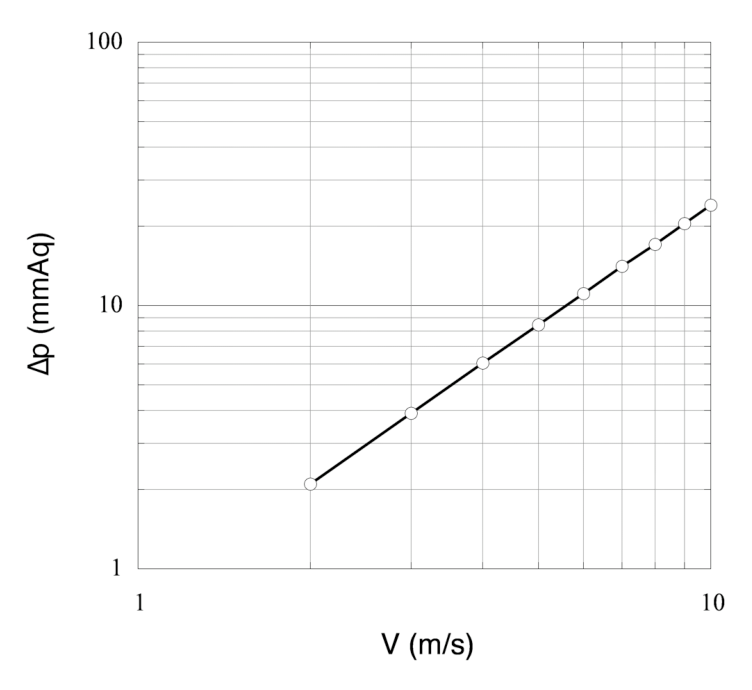
\includegraphics[width=10cm,clip]{ploss.eps}
\end{center}
\caption{$\Delta p-V$性能線図(対数表示)}
\label{fig:ploss}
\end{figure}

\begin{figure}[htdp]
\begin{center}
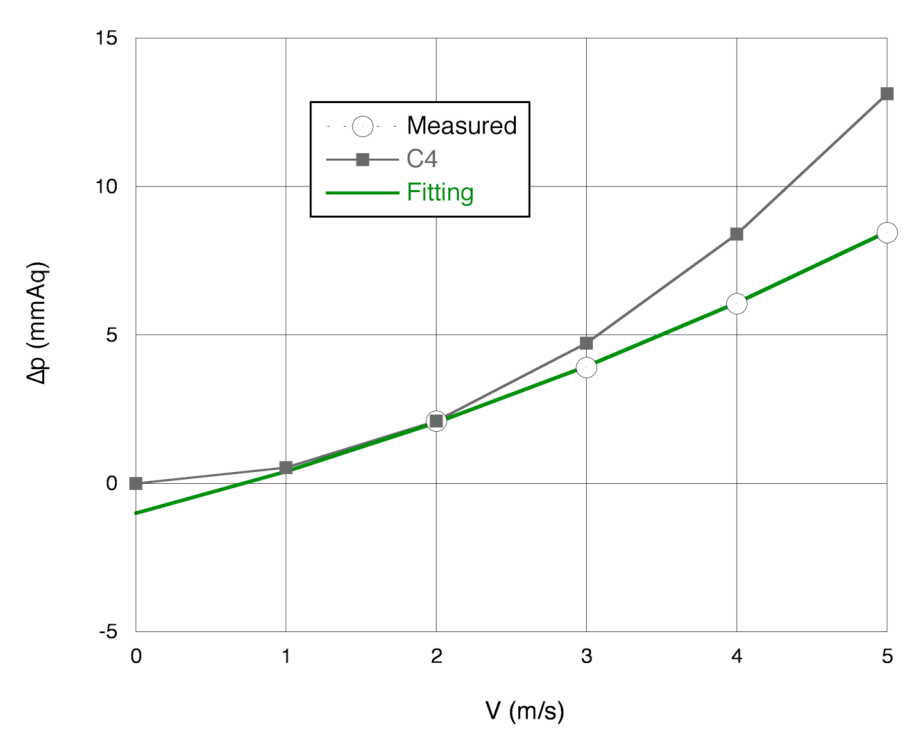
\includegraphics[width=10cm,clip]{rad_para.eps}
\caption{パラメータの取得(\textbf{図\ref{fig:ploss}}と同じものを線形表示)}
\label{fig:get_para}
\end{center}
\end{figure}

\textbf{図\ref{fig:get_para}}に計算パラメータの取得方法を示します.一般に,低速域のデータは得られない場合が多く,推定が必要です.
図では○が測定結果を示し2$[m/s]$より低速域のデータはありません.
そこで,測定値を元にカーブフィッティングを行い(図中の緑色の曲線),算出された係数$c_{1}=0.12321,\,c_{2}=1.2806,\,c_{3}=-1.0074\quad(2-10\,[m/s])$を計算パラメータとします.
この場合,$h'$切片がマイナスになるため,熱交換機の通過速度がゼロに近い場合に急にマイナスの圧力損失(つまり圧力利得)が発生し,実際の現象とは異なり計算上好ましくありません.
そこで\textbf{式(\ref{eq:dp-v})}に示すようにある閾値で曲線を切り替えます.
ここでは,測定された最小速度$u_{threshold}=2\,[m/s]$を閾値として,C4のカーブ$c_{4}=0.525\quad(0-2\,[m/s])$で切り替えます.
熱交換器厚さは実務での観点から単位を$[mm]$で指定するので,注意してください.\\

次の例では,境界条件番号8に圧力損失条件を設定します.
ここで各パラメータは\textbf{表\ref{tbl:ploss_table_ibc}}に対応します.

{\small
\begin{program}
<LocalBoundary>
  <Elem name="Pressure_Loss" ID="8" comment="radiator"/>
    <Param name="Unit"        dtype="STRING" value="mmAq"/>
    <Param name="Normal_x"    dtype="REAL"   value="1.0" />
    <Param name="Normal_y"    dtype="REAL"   value="0.0" />
    <Param name="Normal_z"    dtype="REAL"   value="0.0" />
    <Param name="c1"          dtype="REAL"   value="0.8" />
    <Param name="c2"          dtype="REAL"   value="0.0" />
    <Param name="c3"          dtype="REAL"   value="0.0" />
    <Param name="c4"          dtype="REAL"   value="0.8" />
    <Param name="u_threshold" dtype="REAL"   value="0.2" />
    <Param name="Thickness"   dtype="REAL"   value="80" />
    <Param name="Vector"      dtype="STRING" value="Directional" />
  </Elem>
</LocalBoundary>
\end{program}
}

\begin{table}[htdp]
\caption{圧力損失モデルのパラメータ}
\begin{center}
\small
\begin{tabular}{lll} \toprule
キーワード & パラメータの説明\\ \midrule
Normal\_x & 熱交換器の法線ベクトルのx方向成分\quad 法線は単位ベクトル\\
Normal\_y & 熱交換器の法線ベクトルのy方向成分\quad 法線は単位ベクトル\\
Normal\_z & 熱交換器の法線ベクトルのz方向成分\quad 法線は単位ベクトル\\
c1 & 熱交換器の圧力損失係数\,c1\quad $[mmAq\,|\,mmHg\,|\,Pa\,|\,Non dimension]$\\
c2 & 熱交換器の圧力損失係数\,c2\quad $[mmAq\,|\,mmHg\,|\,Pa\,|\,Non dimension]$\\
c3 & 熱交換器の圧力損失係数\,c3\quad $[mmAq\,|\,mmHg\,|\,Pa\,|\,Non dimension]$\\
c4 & 熱交換器の圧力損失係数\,c4\quad $[mmAq\,|\,mmHg\,|\,Pa\,|\,Non dimension]$\\
u\_threshold & 圧力損失カーブの切り替え速度 $u_{threshold}$ $[m/s\,|\,Non dimension]$\\
thickness & 熱交換器の厚さ\quad $[mm\,|\,Non dimension]$\\
unit & 圧力損失$\Delta p-V$線図のヘッドの単位\quad [$mmAq\,|\,mmHg\,|\,Pa\,|\,Non-Dimension]$ \footnotemark[4]\\
vector & 速度ベクトルの法線方向への強制\quad $[Directional \,|\, Non\_Directional]$\\  \bottomrule
\end{tabular}
\end{center}
\label{tbl:ploss_table_ibc}
\end{table}
\footnotetext[4]{mmAqは水(300K, p=101.325kPa)996.62 $[kg/m^3]$,mmHgは水銀(300K)13538 $[kg/m^3]$をプログラム中でハードコード.}


%%%
\begin{comment}

%
\paragraph{Fan}
\begin{indentation}{3zw}{0zw}
Fanモデル...
\end{indentation}

%
\paragraph{Darcy model}
\label{Darcy model param}
\begin{indentation}{3zw}{0zw}

\ref{sec:porous model}で説明したDarcyモデルでは,等方と非等方モデルが利用できる.透過率パラメータは,\textbf{表\ref{tbl:permeability parameter}}に示すように各主軸方向毎に与える.等方モデルの場合には,各方向のパラメータを同じ値にする.

{ \small
\begin{program}
<Elem name="Forcing_Volume" id="1">
  <Elem name="Darcy" id="50" comment="porous">
    <Param name="permeability_x"  dtype="REAL" value="2.0" />
    <Param name="permeability_y"  dtype="REAL" value="3.0" />
    <Param name="permeability_z"  dtype="REAL" value="4.0" />
  <\Elem>
<\Elem>
\end{program}
}

\begin{table}[htdp]
\caption{Darcyモデルのパラメータ}
\begin{center}
\small
\begin{tabular}{ll} \toprule
キーワード & パラメータの説明\\ \midrule
permeability\_x & x方向の透過率 $[m^2]$\\
permeability\_y & y方向の透過率 $[m^2]$\\
permeability\_z & z方向の透過率 $[m^2]$\\ \bottomrule
\end{tabular}
\end{center}
\label{tbl:permeability parameter}
\end{table}

\end{indentation}

\end{comment}
%%%




%%%
\section{静止座標系と移動座標系の場合の境界条件}
\label{sec:moving_grid}

外部流を考えます.
\textbf{図\ref{fig:reference_frame}}(a)の静止座標系\index{ざひょうけい@座標系!せいし@静止---}と\textbf{図\ref{fig:reference_frame}}(b)の移動座標系\index{ざひょうけい@座標系!いどう@移動---}のように異なる座標系で物体まわりの流れを計算する場合,境界条件の与え方が異なります.
静止座標系は風洞実験に相当し,静止した対象物に対して風をあてている状況です.テストセクション(この場合は計算領域)から出ていく流れが流出風に相当します.
一方,移動座標系では対象物に固定した計算格子が対象物とともに静止流体中を移動します.この場合は,計算領域そのものと内部の格子が物体とともに動きます.
一定速度$V$で動いている座標系の添え字を${}_M$とし,静止した座標系の添え字を${}_S$とします.
いま,静止座標系で観測される流体の速度を$u_{S}$と表すと,同じ速度は移動座標系では$u_{M}-V$のように観測されます.
つまり,
\begin{equation}
u_{S} \, = \, u_{M}-V
\label{eq:galilei}
\end{equation}

\begin{figure}[htbp]
\begin{center}
\subfigure[静止座標系]{
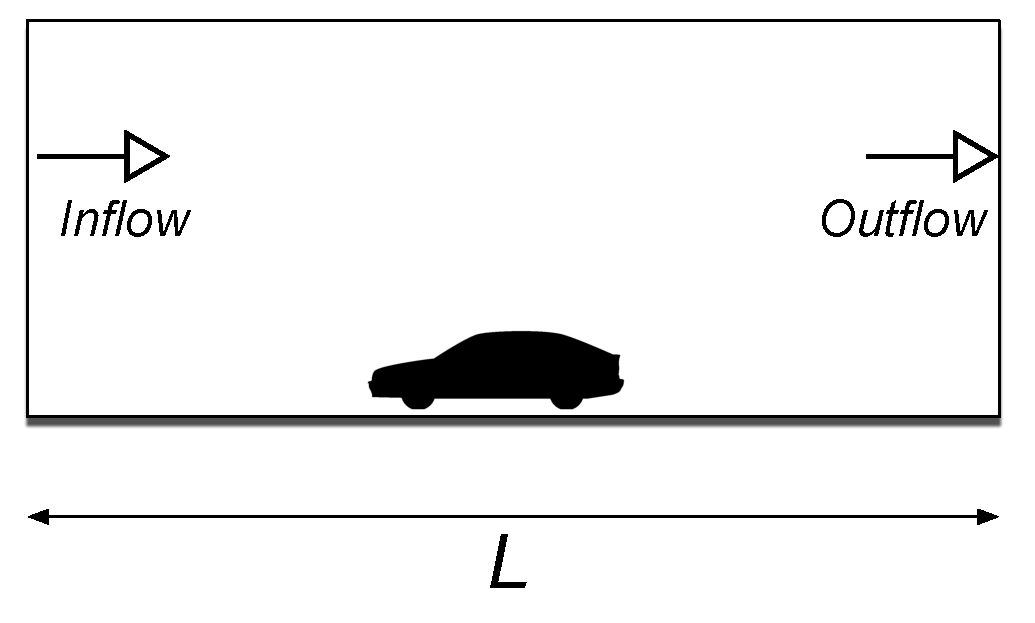
\includegraphics[width=8cm,clip]{stationary.eps}
}
~
\subfigure[移動座標系]{
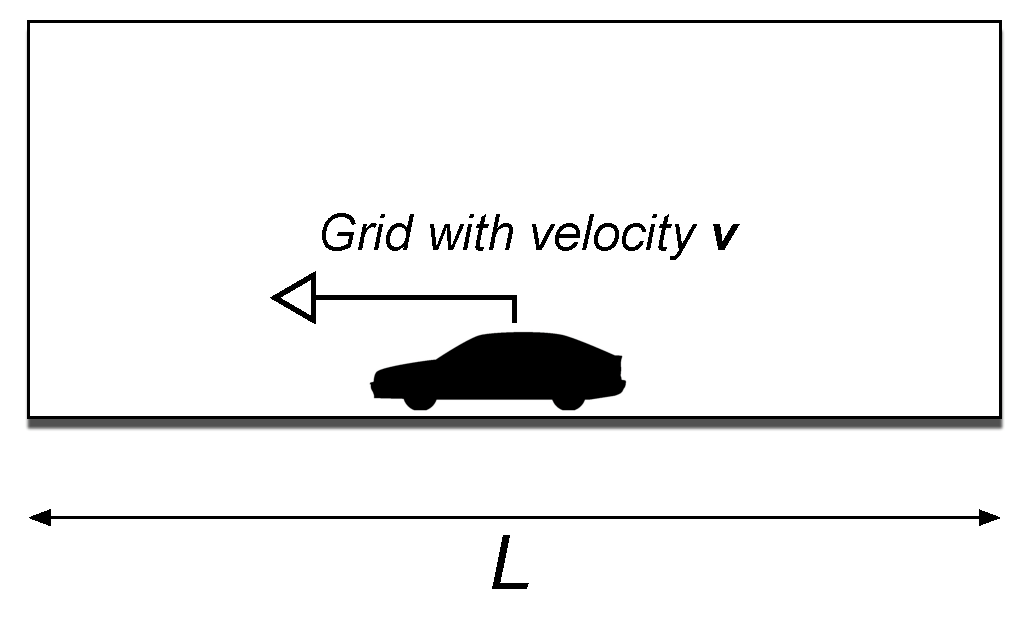
\includegraphics[width=8cm,clip]{moving.eps}
}
\caption{静止座標系と移動座標系の観測点の違い} 
\label{fig:reference_frame}
\end{center}
\end{figure}

静止座標系において\textbf{図\ref{fig:reference_frame}}(a)のような境界条件を与える場合,流入部では$u_{0}$を与えます.
一方,移動座標系では静止流体の条件,つまり$u=0,\,p=0$を想定し,格子速度$V=-u_{0}$を与えると両者は等価になります.

移動座標系の場合注意を要するのが,物体と地面の境界条件です.物体は移動しているので格子速度と同じになります.
一方,地面は静止している地面と動いている地面の二通りが考えられます.
前者は風洞実験で固定地面板に相当し,後者はムービングベルトに相当します.
ムービングベルトの場合には物体と格子速度だけ相対速度をもっていることになります.
したがって,

\begin{equation}
u_{ground}\,=\,
\begin{cases}
\, -u_{0} & \quad (Stationary\,ground)\\
\, 0 & \quad (Moving\,ground)\\
\end{cases}
\label{eq:relative velocity wall}
\end{equation}

移動格子の移動速度は\hyperlink{tgt:reference_frame}{Reference\_Frame}セクションで与えます.





